\begin{figure*}[t]\centering
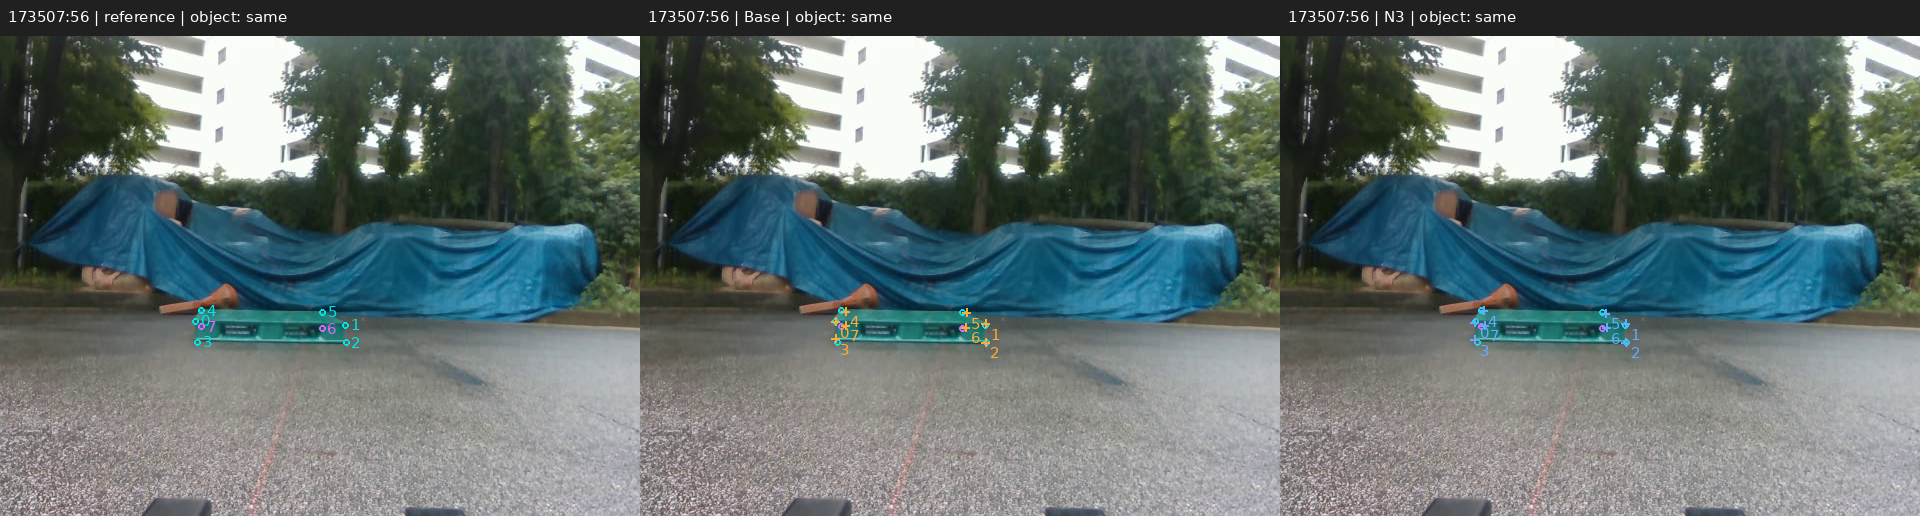
\includegraphics[width=.97\textwidth]{figures/pnp_assisted_lifter_12/173507_56.png}\par\smallskip
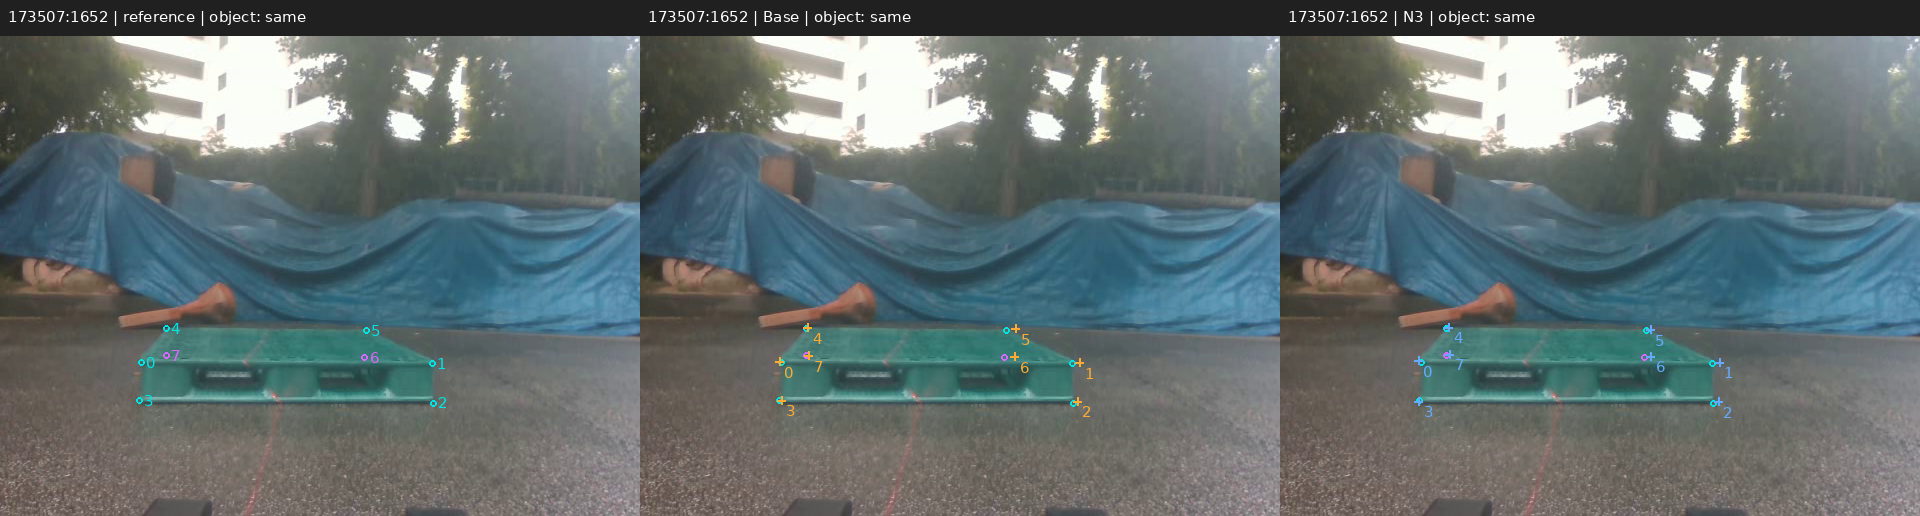
\includegraphics[width=.97\textwidth]{figures/pnp_assisted_lifter_12/173507_1652.png}\par\smallskip
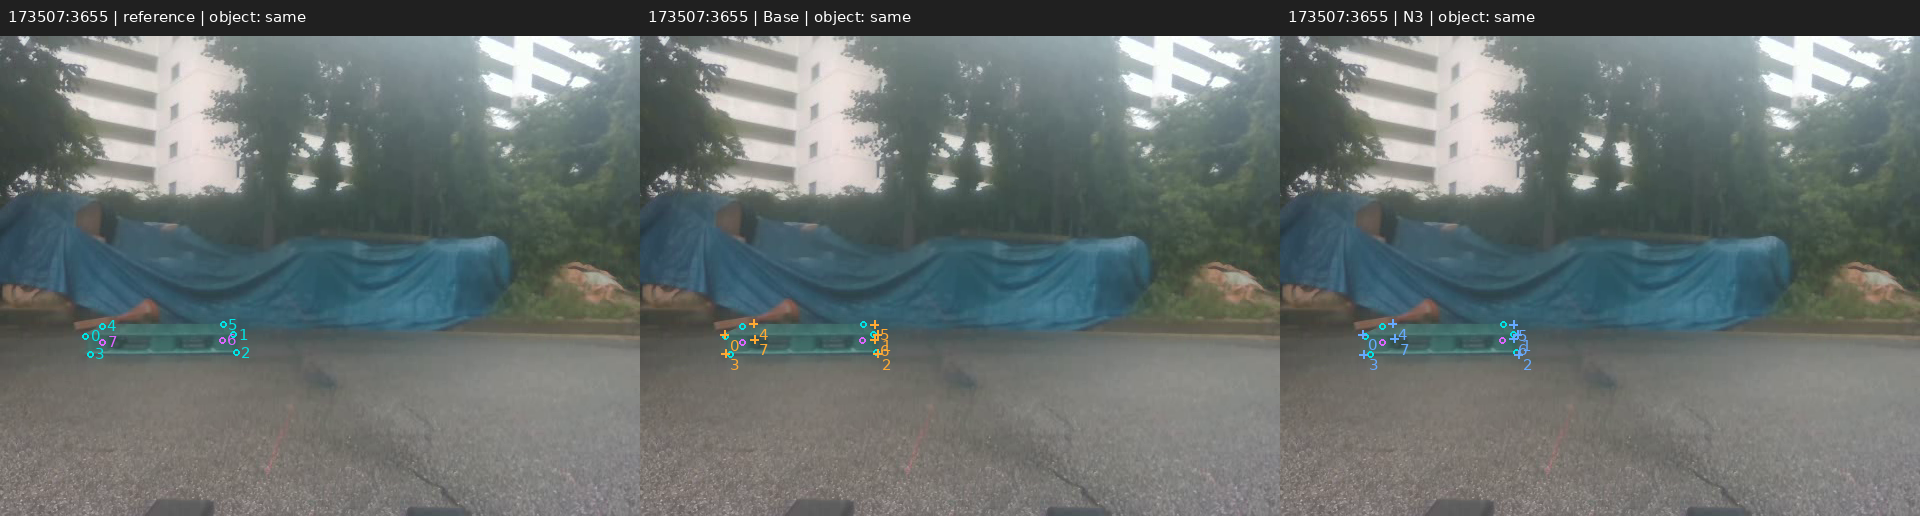
\includegraphics[width=.97\textwidth]{figures/pnp_assisted_lifter_12/173507_3655.png}\par\smallskip
\caption{173507세션의 사전 고정 3장 전체. 왼쪽은 원래 기하 참조(청록 직접 클릭·보라 PnP), 가운데 Base, 오른쪽 N3이다. 생성 경로를 표시하며 독립 물리 정답이나 모든 점의 직접 가시성을 뜻하지 않는다.}\label{sup:lifter_assisted_173507}
\end{figure*}
\begin{figure*}[t]\centering
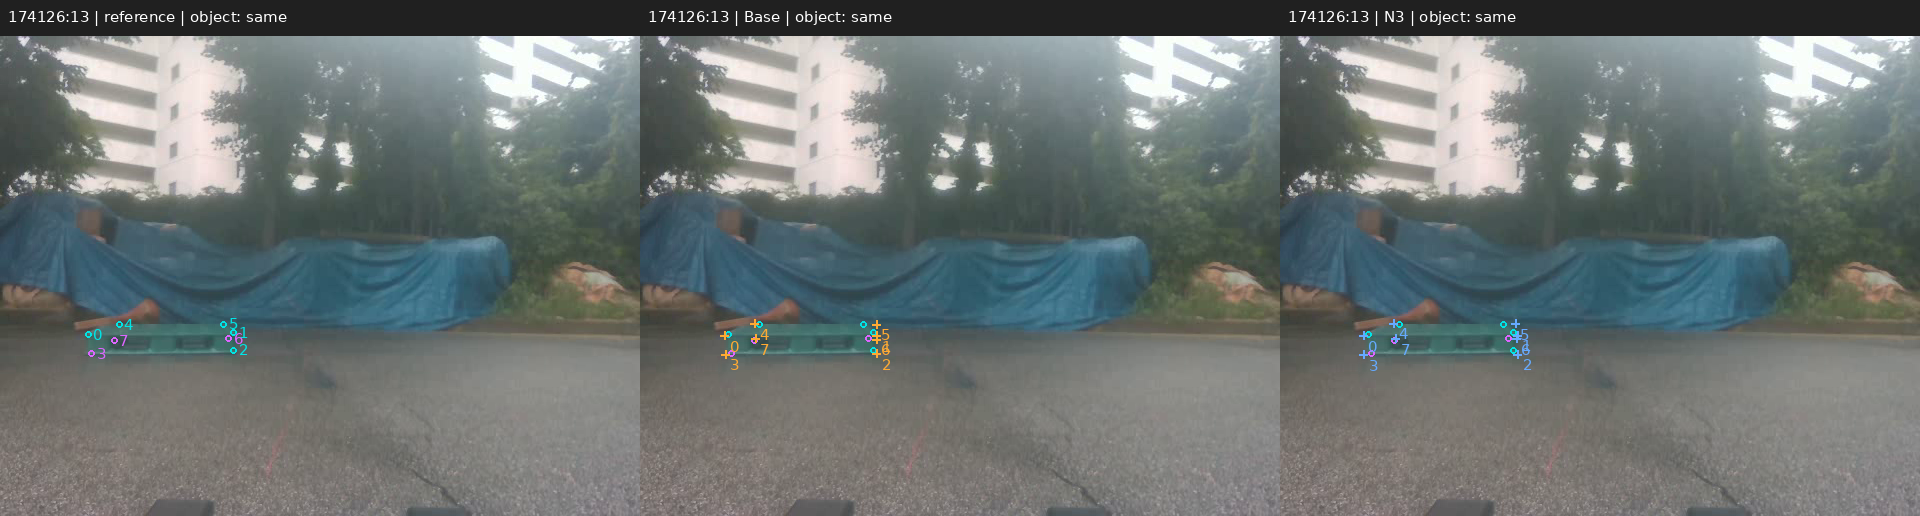
\includegraphics[width=.97\textwidth]{figures/pnp_assisted_lifter_12/174126_13.png}\par\smallskip
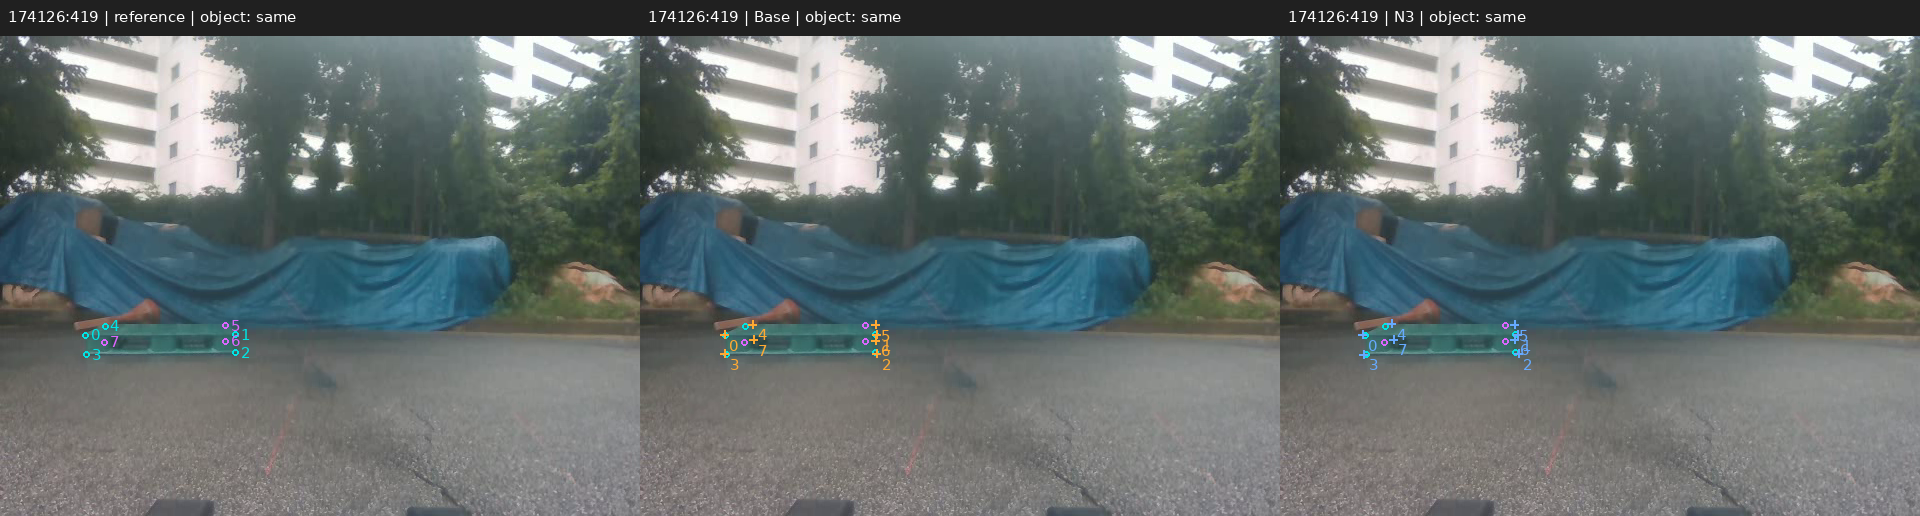
\includegraphics[width=.97\textwidth]{figures/pnp_assisted_lifter_12/174126_419.png}\par\smallskip
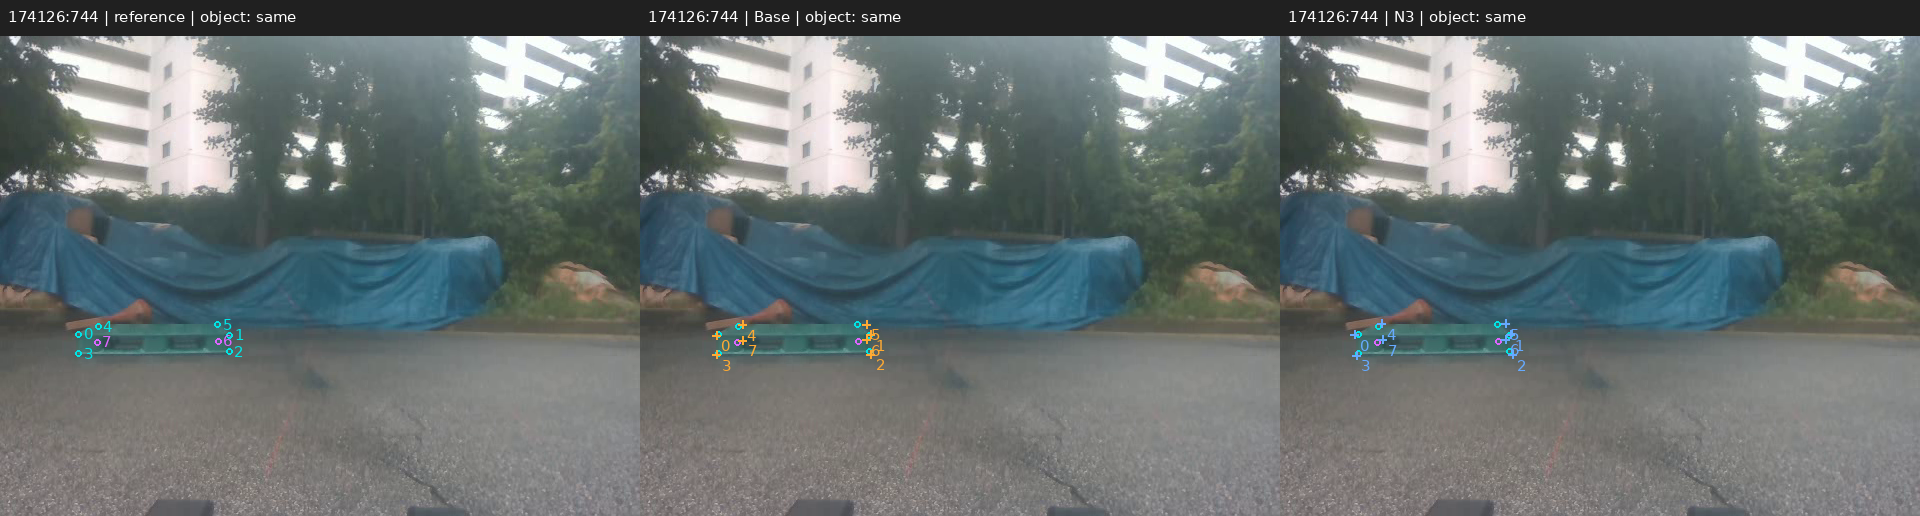
\includegraphics[width=.97\textwidth]{figures/pnp_assisted_lifter_12/174126_744.png}\par\smallskip
\caption{174126세션의 사전 고정 3장 전체. 왼쪽은 원래 기하 참조(청록 직접 클릭·보라 PnP), 가운데 Base, 오른쪽 N3이다. 생성 경로를 표시하며 독립 물리 정답이나 모든 점의 직접 가시성을 뜻하지 않는다.}\label{sup:lifter_assisted_174126}
\end{figure*}
\begin{figure*}[t]\centering
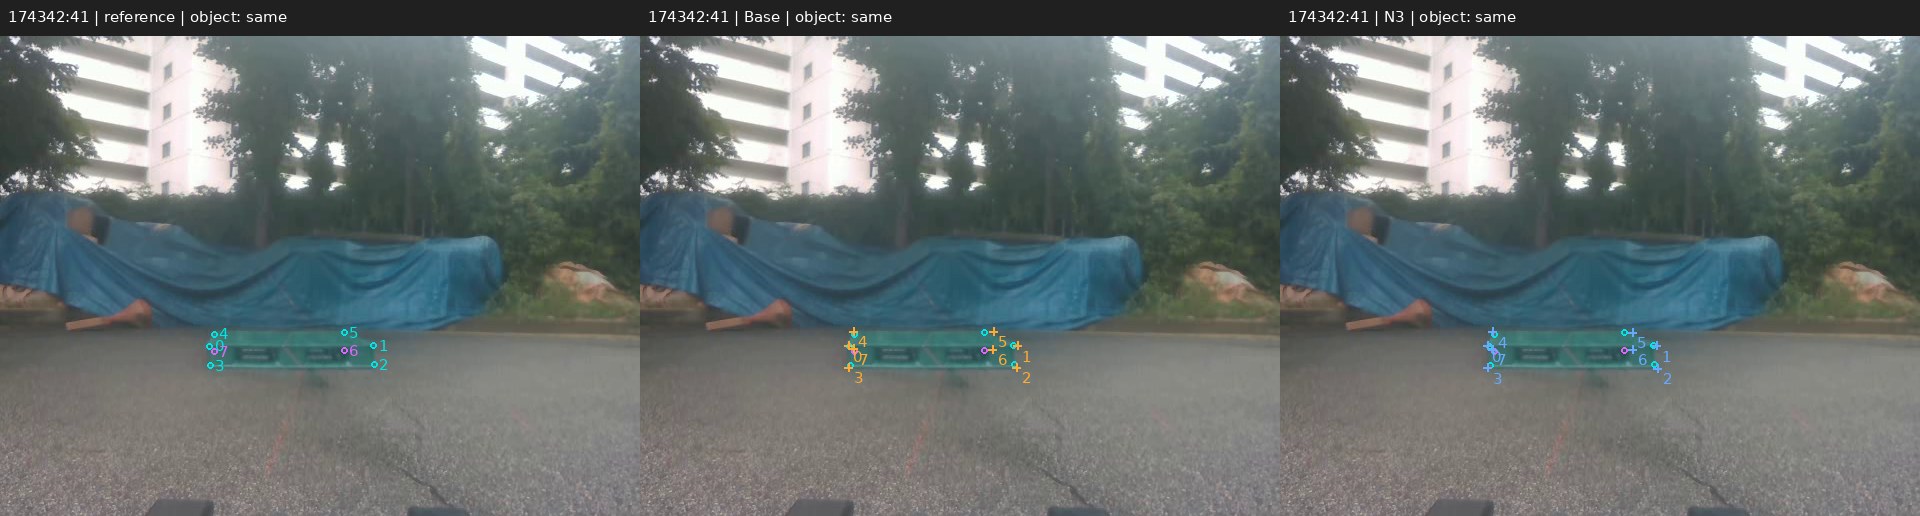
\includegraphics[width=.97\textwidth]{figures/pnp_assisted_lifter_12/174342_41.png}\par\smallskip
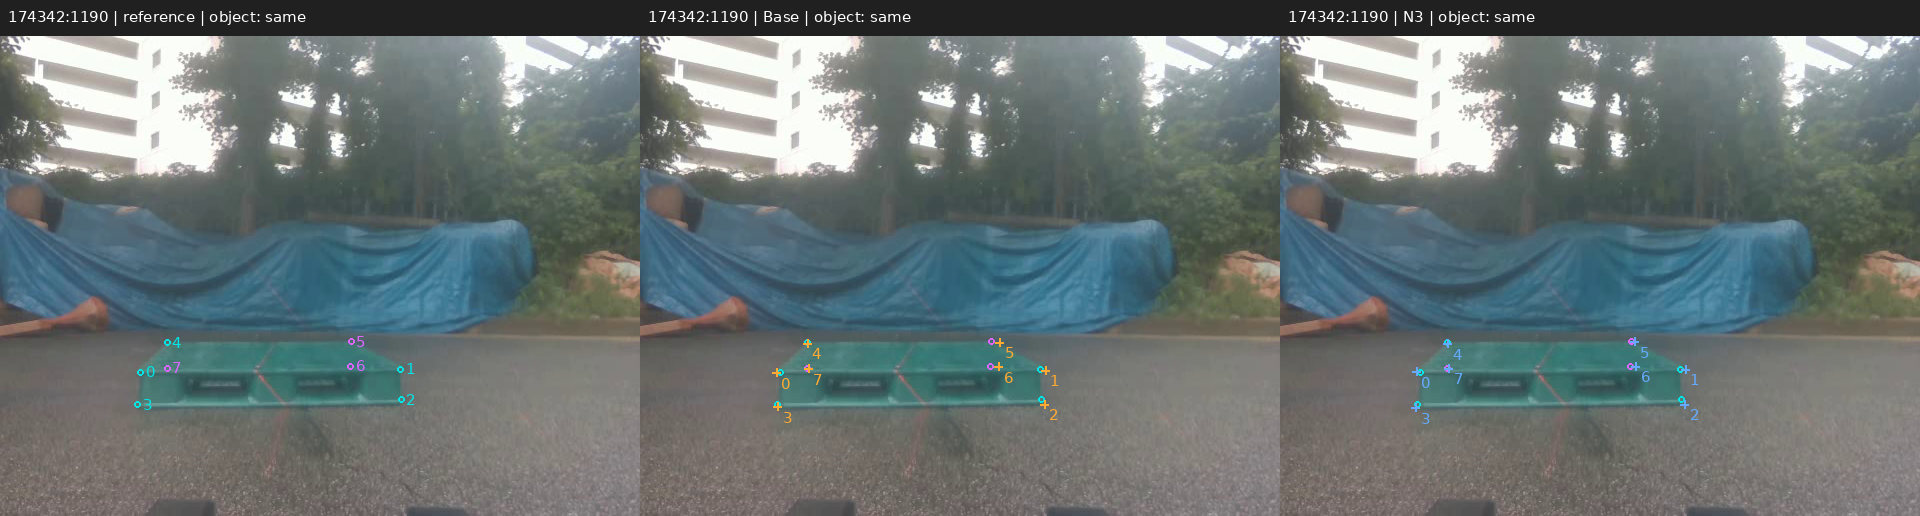
\includegraphics[width=.97\textwidth]{figures/pnp_assisted_lifter_12/174342_1190.png}\par\smallskip
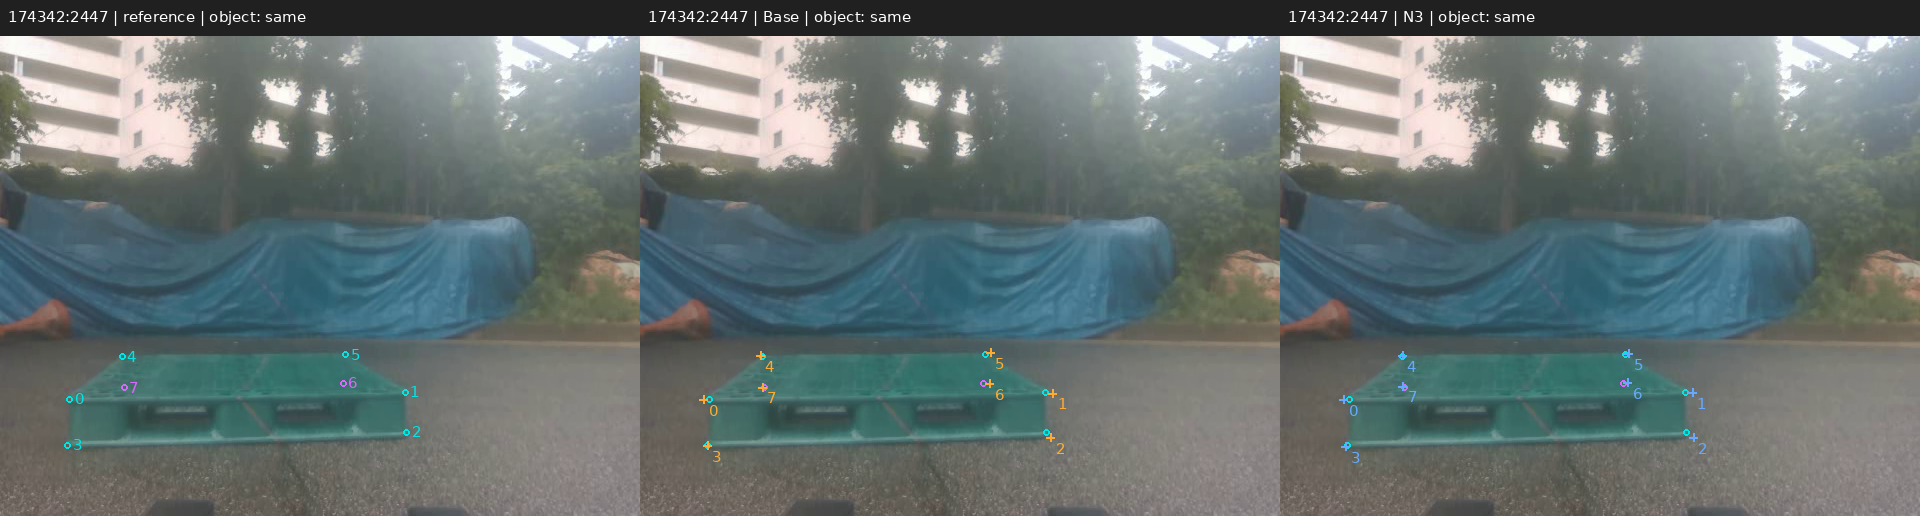
\includegraphics[width=.97\textwidth]{figures/pnp_assisted_lifter_12/174342_2447.png}\par\smallskip
\caption{174342세션의 사전 고정 3장 전체. 왼쪽은 원래 기하 참조(청록 직접 클릭·보라 PnP), 가운데 Base, 오른쪽 N3이다. 생성 경로를 표시하며 독립 물리 정답이나 모든 점의 직접 가시성을 뜻하지 않는다.}\label{sup:lifter_assisted_174342}
\end{figure*}
\begin{figure*}[t]\centering
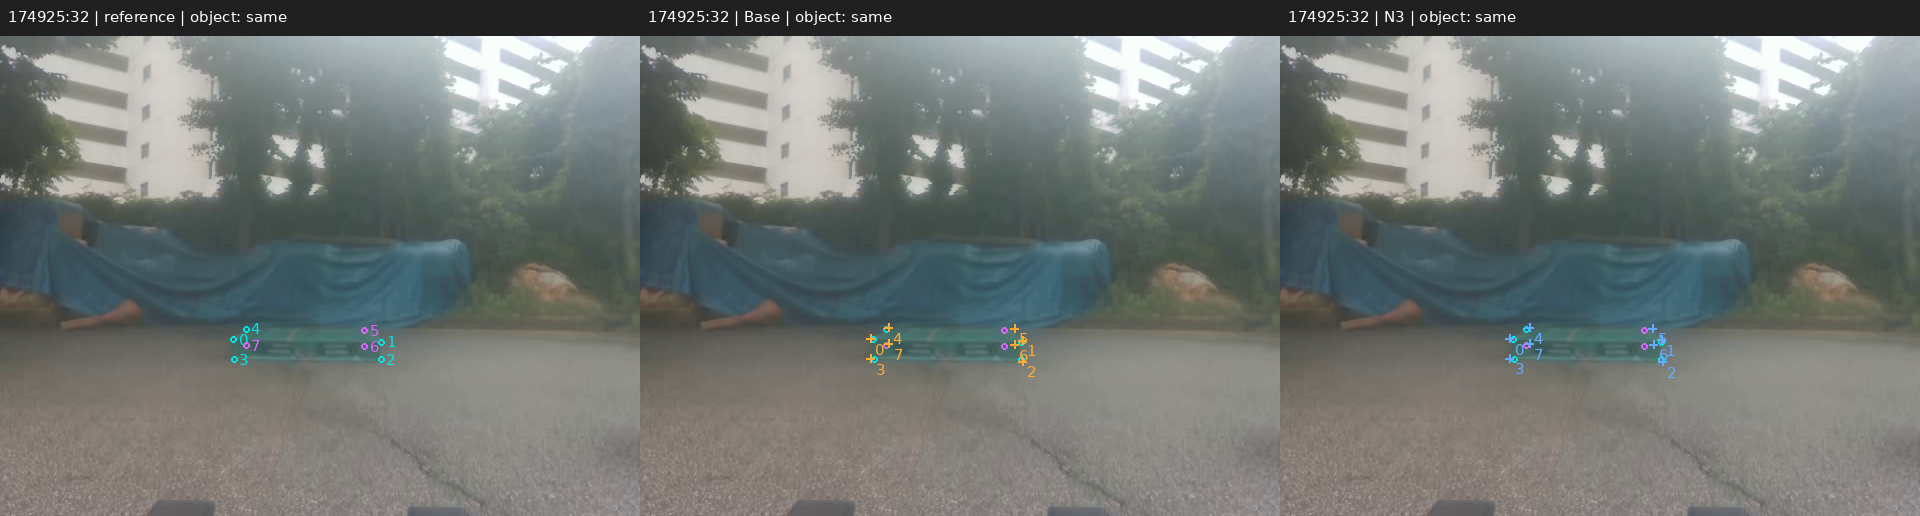
\includegraphics[width=.97\textwidth]{figures/pnp_assisted_lifter_12/174925_32.png}\par\smallskip
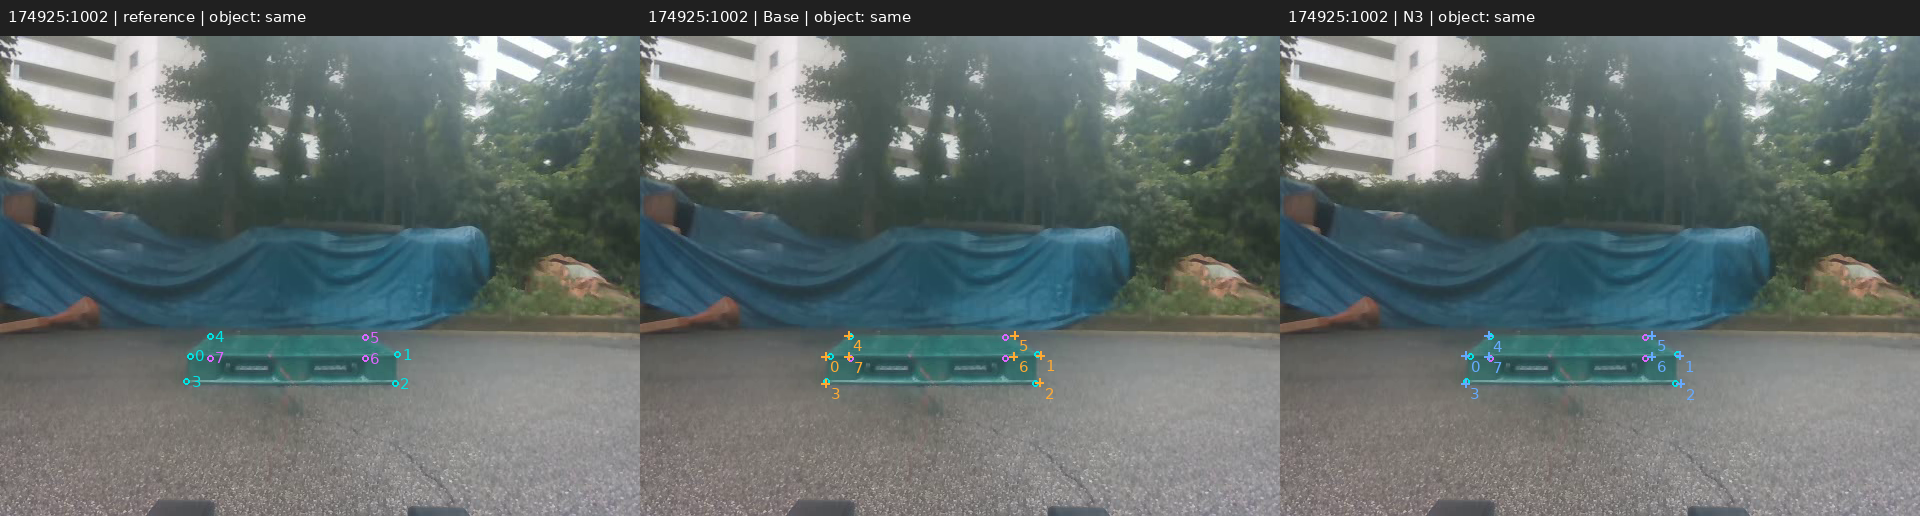
\includegraphics[width=.97\textwidth]{figures/pnp_assisted_lifter_12/174925_1002.png}\par\smallskip
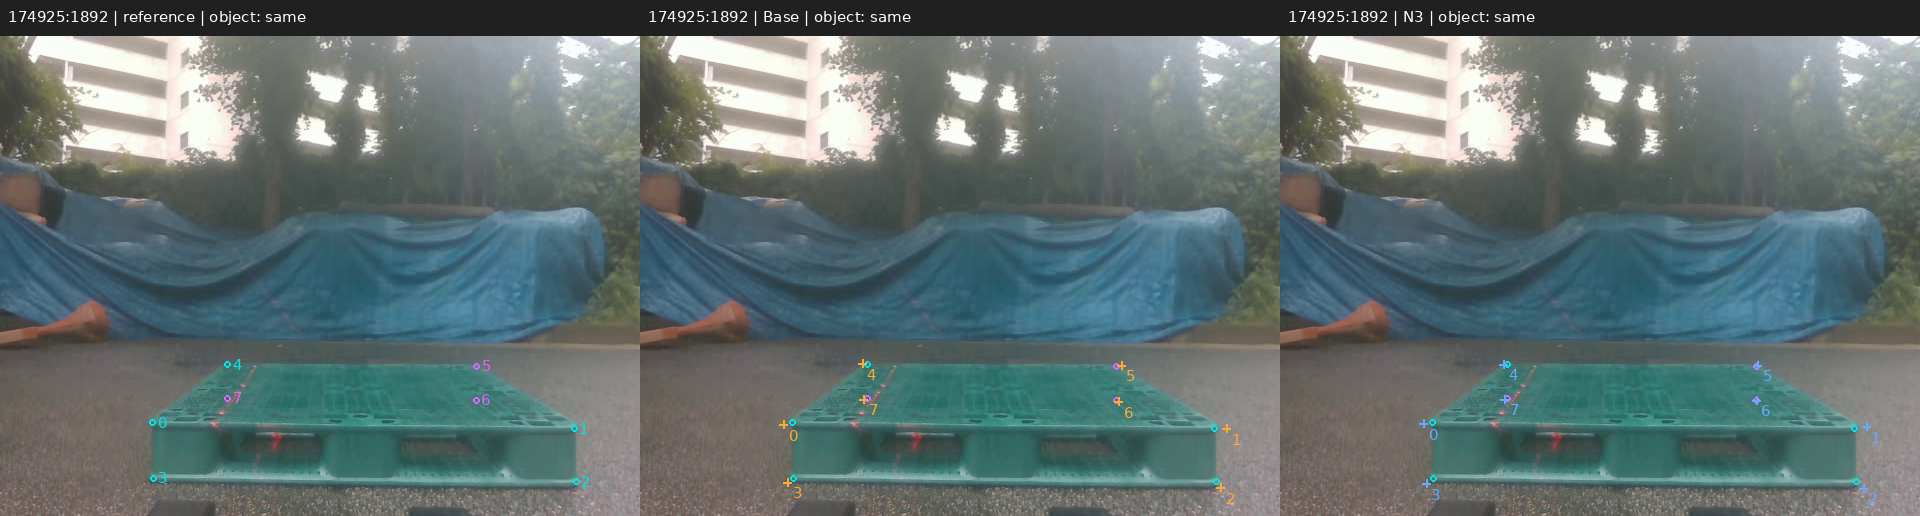
\includegraphics[width=.97\textwidth]{figures/pnp_assisted_lifter_12/174925_1892.png}\par\smallskip
\caption{174925세션의 사전 고정 3장 전체. 왼쪽은 원래 기하 참조(청록 직접 클릭·보라 PnP), 가운데 Base, 오른쪽 N3이다. 생성 경로를 표시하며 독립 물리 정답이나 모든 점의 직접 가시성을 뜻하지 않는다.}\label{sup:lifter_assisted_174925}
\end{figure*}
